\documentclass[handout]{beamer} 
\title{ITCS 532:\\ 
3. Universal Turing Machines}
\date{}
\author{Rob Egrot}

\usepackage{amsmath, bbold, bussproofs,graphicx}
\usepackage{mathrsfs}
\usepackage{amsthm}
\usepackage{amssymb}
\usepackage[all]{xy}
\usepackage{multirow}
\usepackage{tikz-cd}


\newtheorem{proposition}[theorem]{Proposition}
\newcommand{\bN}{\mathbb{N}}
\newcommand{\bZ}{\mathbb{Z}}
\newcommand{\bQ}{\mathbb{Q}}
\newcommand{\bR}{\mathbb{R}}
\newcommand{\bP}{\mathbb{P}}
\newcommand{\tvs}{\textvisiblespace}
\newcommand{\ra}{\rightarrow}
\newcommand{\la}{\leftarrow}
\newcommand{\co}{\mathbf{code}}

\addtobeamertemplate{navigation symbols}{}{%
    \usebeamerfont{footline}%
    \usebeamercolor[fg]{footline}%
    \hspace{1em}%
    \insertframenumber/\inserttotalframenumber
}
\setbeamertemplate{theorems}[numbered]
\begin{document}

\begin{frame}
\titlepage
\end{frame}

\begin{frame}
\frametitle{Universal Computation}
\begin{itemize}
\item Machines for computation have existed for thousands of years. E.g.
\begin{itemize}
\item The Antikythera mechanism from 1st or 2nd century BC Greece.
\item The Banu Musa brothers' automatic mechanical flute player from 9th century Persia.
\end{itemize} 
\item These devices can compute, but they cannot \emph{simulate}.
\item I.e. a modern computer can mimic the calculations of the Antikythera mechanism, but the Antikythera mechanism can't run Windows.
\item The first \emph{universal} computer design was probably the Analytical Engine by Charles Babbage and Ada Lovelace in 1837.
\item This was never built due to cost, but it would, in theory, have been able to run Windows.
\end{itemize}
\end{frame}

\begin{frame}
\frametitle{Difference Engine no. 2}
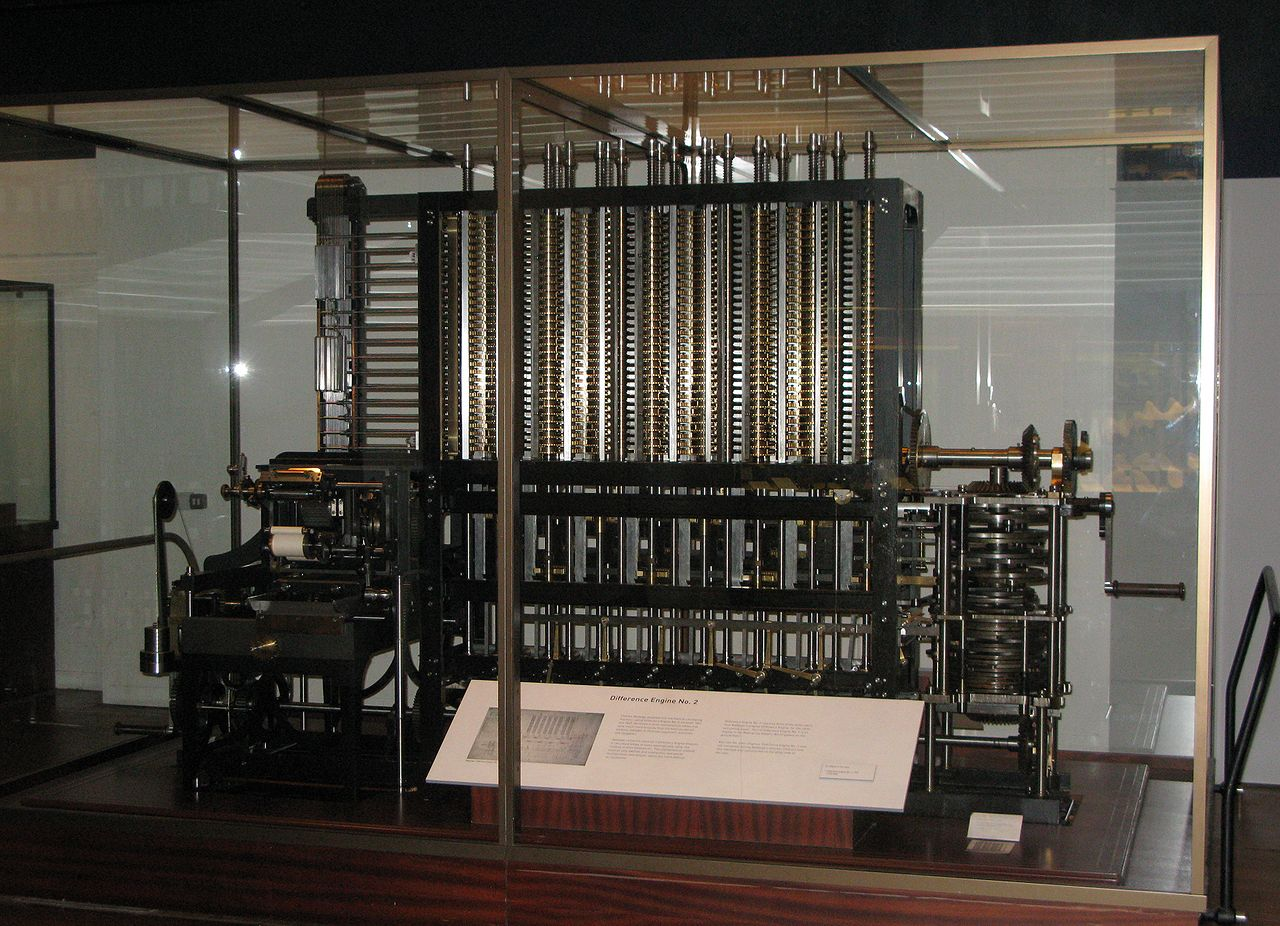
\includegraphics[scale = 0.22]{DE2.jpg}  

The Difference Engine no. 2. Photo from Wikipedia (https://commons.wikimedia.org/w/index.php?curid=4807331)
\end{frame}

\begin{frame}
\frametitle{Universal Computation with Turing Machines}
\begin{itemize}
\item Babbage and Lovelace did not have the theoretical framework to understand universal computation.
\vspace{0.3cm}
\item But we do, because we know about Turing machines.
\vspace{0.3cm}
\item Remember that a Turing machine is defined by a $5$-tuple $(Q,\Sigma,q_0,H,\delta)$.
\vspace{0.3cm}
\item We've been defining alphabets and states on an ad hoc basis, but we can make our approach more systematic by unifying our choice of symbols.
\vspace{0.3cm}
\item Define $\hat{\Sigma}=\{\sigma_0,\sigma_1,\sigma_2,\ldots\}$ and $\hat{Q}=\{q_0,q_1,q_2,\ldots\}$.
\vspace{0.3cm}
\item This is enough to define any TM.
\end{itemize}
\end{frame}

\begin{frame}
\frametitle{Encoding Turing Machines}
\begin{itemize}
\item Given a TM defined by $(Q,\Sigma,q_0,H,\delta)$ we can assume:
\vspace{0.2cm}
\item $Q$ is a finite subset of $\hat{Q}$, $\Sigma$ is a finite subset of $\hat{\Sigma}$. 
\vspace{0.2cm}
\item $q_0$ is just $q_0$ from $\hat{Q}$. 
\vspace{0.2cm}
\item $:$, $\tvs$, $\la$, and $\ra$ are $\sigma_0$, $\sigma_1$, $\sigma_2$, and $\sigma_3$ from $\hat{\Sigma}$ respectively.
\vspace{0.2cm}
\item Every Turing machine is specified by a finite subset of $\hat{Q}\cup\hat{\Sigma}$, along with a transition function $\delta$ that is formally a finite subset of $\hat{Q}\times\hat{\Sigma}\times\hat{Q}\times\hat{\Sigma}$. 
\vspace{0.2cm}
\item So the set of all Turing machines corresponds to a subset of the set of all finite subsets of a countable set, and so is countable. 
\vspace{0.2cm}
\item I.e. there's a 1-1 function $\co$  from the set of all Turing machines to $\{0,1\}^*$.
\end{itemize}
\end{frame}

\begin{frame}
\frametitle{Defining a $\co$ function - symbols and states}
\begin{itemize}
\item There are many ways we can define a $\co$ function.
\item Here is one example.
\item For $q_n$ we define $\co(q_n)$ to be $n+1$ `1' symbols. So, e.g. $\co(q_2)=111$.
\item For $\sigma_n$ we define $\co(\sigma_n)$ to be $n+1$ `1' symbols. So, e.g. $\co(\sigma_1)=11$.
\item Given a Turing machine $T$ with states $Q=\{q_0,\ldots,q_m\}$ and alphabet $\Sigma=\{\sigma_0,\ldots,\sigma_n\}$ we define the strings 
\begin{equation*}\co(Q)=\co(q_0)0\co(q_1)0\ldots0\co(q_m)0\end{equation*}
and
\begin{equation*}\co(\Sigma)=\co(\sigma_0)0\co(\sigma_1)0\ldots0\co(\sigma_n)0\end{equation*}
\end{itemize}
\end{frame}

\begin{frame}
\frametitle{Defining a $\co$ function - accept and reject}
\begin{itemize}
\item Let $q_i$ and $q_j$ be the accept and reject states respectively. 
\vspace{0.7cm}
\item The concatenated string \[\co(Q)0\co(\Sigma)0\co(q_i)0\co(q_j)0\] encodes the states and alphabet that define $T$.
\vspace{0.7cm}
\item All that is left is to find a way to encode $\delta$.
\end{itemize}
\end{frame}

\begin{frame}
\frametitle{Defining a $\co$ function - $\delta$}
\begin{itemize}
\item $\delta$ is formally defined as a set of tuples $(q,\sigma,q',\sigma')$. We can code a tuple $t=(q,\sigma,q',\sigma')$ as 
\begin{equation*}\co(t)=\co(q)0\co(\sigma)0\co(q')0\co(\sigma')0\end{equation*} 
\vspace{0.2cm}
\item If $\delta$ is defined by tuples $t_1,t_2,\ldots,t_k$ we can define 
\begin{equation*}\co(\delta)=\co(t_1)\co(t_2)\ldots \co(t_k)\end{equation*}
\vspace{0.2cm}
\item Note that this is not strictly speaking well defined, because it depends on the order of the tuples $\delta$.
\vspace{0.2cm}
\item To avoid this problem we assume a canonical ordering (something like alphabetical).
\end{itemize}
\end{frame}

\begin{frame}
\frametitle{Defining a $\co$ function - putting it all together}
\begin{itemize}
\item Combining all this we can encode $T$ with 
\begin{equation*}\co(T)= \co(Q)0\co(\Sigma)0\co(q_i)0\co(q_j)0\co(\delta)\end{equation*}
\vspace{0.2cm}
\item If $I$ is a string defined by $I=\sigma'_1\sigma'_2\ldots\sigma'_l$ (where the $\sigma'$ are symbols from $\hat{\Sigma}$) we can encode $I$ using 
\begin{equation*}\co(I)=\co(\sigma'_1)0\co(\sigma'_2)0\ldots 0\co(\sigma'_l)\end{equation*}
\vspace{0.2cm}
\item We can encode the pair $(T,I)$ representing the Turing machine $T$ and input $I$ using 
\begin{equation*}\co(T,I)=\co(T)00\co(I)\end{equation*}
\end{itemize}
\end{frame}

\begin{frame}
\frametitle{Example}
Alphabet $\Sigma=\{:,\tvs,a,b\}$, machine adds $a$ to the end of its input.
\begin{center}
\begin{tikzpicture}[scale=0.2]
\tikzstyle{every node}+=[inner sep=0pt]
\draw [black] (9.4,-31.3) circle (3);
\draw (9.4,-31.3) node {$q_0$};
\draw [black] (22.4,-31.3) circle (3);
\draw (22.4,-31.3) node {$q_1$};
\draw [black] (36,-31.6) circle (3);
\draw (36,-31.6) node {$q_2$};
\draw [black] (36,-31.6) circle (2.4);
\draw [black] (22.4,-44.4) circle (3);
\draw (22.4,-44.4) node {$q_3$};
\draw [black] (22.4,-44.4) circle (2.4);
\draw [black] (12.4,-31.3) -- (19.4,-31.3);
\fill [black] (19.4,-31.3) -- (18.6,-30.8) -- (18.6,-31.8);
\draw (15.9,-31.8) node [below] {$:,\ra$};
\draw [black] (25.4,-31.37) -- (33,-31.53);
\fill [black] (33,-31.53) -- (32.21,-31.02) -- (32.19,-32.02);
\draw (29.17,-32.01) node [below] {$\tvs,a$};
\draw [black] (22.4,-34.3) -- (22.4,-41.4);
\fill [black] (22.4,-41.4) -- (22.9,-40.6) -- (21.9,-40.6);
\draw (21.9,-37.85) node [left] {$:,\ra$};
\draw [black] (11.51,-33.43) -- (20.29,-42.27);
\fill [black] (20.29,-42.27) -- (20.08,-41.35) -- (19.37,-42.05);
\draw (15.38,-39.33) node [left] {$\{a,b,\tvs\},\tvs$};
\draw [black] (21.077,-28.62) arc (234:-54:2.25);
\draw (22.4,-24.05) node [above] {$\{a,b\},\ra$};
\fill [black] (23.72,-28.62) -- (24.6,-28.27) -- (23.79,-27.68);
\end{tikzpicture}
\end{center}
The accept state is $q_2$, and the reject state is $q_3$. To encode this machine we first assign $a$ and $b$ correspondents in $\hat{\Sigma}$. We'll say $a=\sigma_4$ and $b=\sigma_5$ (because $:=\sigma_0$, $\tvs=\sigma_1$, $\la=\sigma_2$, and $\ra=\sigma_3$).
\end{frame}

\begin{frame}
\frametitle{Example - the formal transition function}
The transition function $\delta$ is then defined by the tuples
\begin{align*}
(q_0,:,q_1,\ra)&=(q_0,\sigma_0,q_1,\sigma_3)\\
(q_0,\tvs,q_3,\tvs)&=(q_0,\sigma_1,q_3,\sigma_1)\\
(q_0,a,q_3,\tvs)&=(q_0,\sigma_4,q_3,\sigma_1)\\
(q_0,b,q_3,\tvs)&=(q_0,\sigma_5,q_3,\sigma_1)\\
(q_1,:,q_3,\ra)&=(q_1,\sigma_0,q_3,\sigma_1)\\
(q_1,a,q_1,\ra)&=(q_1,\sigma_4,q_1,\sigma_3)\\
(q_1,b,q_1,\ra)&=(q_1,\sigma_5,q_1,\sigma_3)\\
(q_1,\tvs,q_2,a)&=(q_1,\sigma_1,q_2,\sigma_4)\\
\end{align*}
Note that I didn't put these tuples into alphabetical order first. Technically this is wrong, but we won't worry about that here!
\end{frame}

\begin{frame}
\frametitle{Example - the coded form}
So using our definitions we get 
\begin{itemize}
\item $\co(Q)=10110111011110$
\item $\co(\Sigma)=101101110111101111101111110$
\item $\co(q_i)=111$
\item $\co(q_j)=1111$
\item Finally \begin{align*}\co(\delta)=&1010110111101011011110110101111101111011010 \\
                                        &1111110111101101101011110110110111110110111 \\
																				&101101111110110111101101101110111110\end{align*}
\item And so \begin{align*} \co(T)=     &1011011101111001011011101111011111011111100 \\
                                        &1110111101010110111101011011110110101111101\\
																				&1110110101111110111101101101011110110110111\\
																				&110110111101101111110110111101101101110111110                                    																
                                       \end{align*}
\end{itemize}
\end{frame}

\begin{frame}
\frametitle{Universal Turing Machines}
\begin{itemize}
\item We can code Turing machines and inputs as finite strings over the alphabet $\{0,1\}$.
\vspace{0.1cm}
\item Turing machines can manipulate finite strings. 
\vspace{0.1cm}
\item Therefore we can create Turing machines that act on the codes of other Turing machines.
\vspace{0.1cm}
\item We're interested in TMs that \emph{simulate} the action of another TM on an input. 
\vspace{0.1cm}
\item A Turing machine that can do this is called \emph{universal}. 
\vspace{0.1cm}
\item More precisely, if $U$ is a universal Turing machine (UTM), $T$ is any other TM, and $I$ is an input for $T$, then:
\begin{itemize} 
\item $U(\co(T,I))$ halts if and only if $T(I)$ halts (and accepts or rejects appropriately). 
\item The output of $U(\co(T,I))$ is the coded form of the output of $T(I)$.
\end{itemize}
\end{itemize}
\end{frame}

\begin{frame}
\frametitle{Designing a Universal Turing Machine}
\begin{itemize}
\item We will use a 3-tape machine.
\vspace{0.3cm}
\item We know that if this exists there's a 1-tape machine that does the same thing.
\vspace{0.3cm}
\item The 1st tape is used for input and output. It starts with $\co(T,I)$ written on it (where $T$ is the machine to be simulated on input $I$). Later in the calculation it will store the state of the tape of $T$ in coded form.
\vspace{0.3cm}
\item The 2nd tape will be used to store $\co(T)$ for reference.
\vspace{0.3cm}
\item The 3rd tape will be used to store the coded form of the state of $T$.
\end{itemize} 
\end{frame}

\begin{frame}
\frametitle{Running our UTM - starting up}
A run of this machine $U$ on input $\co(T,I)$ starts as follows:
\vspace{0.3cm}
\begin{enumerate}
\item $U$ copies $\co(T)$ from tape 1 onto tape 2.
\vspace{0.3cm}
\item $U$ erases $\co(T)$ from tape 1 and shifts $\co(I)$ to the start of the tape so tape 1 just contains $\co(I)$.
\vspace{0.3cm}
\item $U$ writes $\co(q_0)$ on tape 3.
\end{enumerate}
\end{frame}

\begin{frame}
\frametitle{Running our UTM - simulating a step}
The simulation of a single step of $T(I)$ by $U$ goes as follows:

\begin{enumerate}
\item $U$ searches tape 2 for an instruction corresponding to the state of the machine coded on tape 3 and the symbol currently being read in coded form on tape 1. 
\begin{itemize}
\item E.g. symbol being read by $T$ corresponds to string of ones to the left of zero being read by $U$. 
\end{itemize}
\item Based on the instruction it updates tape 3 to represent the new state of $T$, and updates tape 1 to represent the new contents of the tape of $T$ and the new position of the tape head.
\item If $T$ has reached a halt state then $U$ halts in the corresponding halt state, otherwise $U$ goes back to 1.
\end{enumerate}
\end{frame}

\begin{frame}
\frametitle{The Existence of Undecidable problems}
\begin{itemize} 
\item Every decision problem corresponds to a formal language. 
\item Given a finite alphabet $\Sigma$ the set $\Sigma^*$, is countably infinite. 
\item The formal languages over $\Sigma$ are the subsets of $\Sigma^*$, so the set of all formal languages over $\Sigma$ is $\wp(\Sigma^*)$, which is uncountable.\
\item Every Turing machine can be represented by a finite string over the alphabet $\{0,1\}$. 
\item So the set of all distinct Turing machines is a subset of the set of all finite strings over $\{0,1\}$, i.e. $\{0,1\}^*$, which is countably infinite. 
\item So there must be (many) more formal languages (and so decision problems) than there are Turing machines capable of deciding them! 
\item There must be decision problems which cannot be decided (or semidecided) by a Turing machine. 
\end{itemize}
\end{frame}

\begin{frame}
\frametitle{Universal Computers in the Wild}
\begin{itemize} 
\item It turns out that abstract universal computers are actually very common. 
\vspace{0.7cm}
\item Many if not most deterministic processes that are not obviously trivial turn out to be capable of universal computation.
\vspace{0.3cm}
\begin{itemize}
\item In the sense that you can decide rules for input and output that let you simulate Turing machines (including UTMS). 
\end{itemize}
\vspace{0.3cm}
\item We will look at some examples now.
\end{itemize}
\end{frame}

\begin{frame}
\frametitle{Rule 110}
\begin{itemize}
\item An elementary cellular automaton consists of a 2-way infinite tape whose cells can contain either 0 or 1. 
\item At each step of a computation the contents of a cell changes based on its contents and the contents of its immediate neighbours. 
\item Rule 110 is an elementary cellular automaton with update rules described in the following table.
\begin{center}
\tiny
\begin{tabular}{| c |c |c |c |c |c |c |c |c|}
\hline
 Cell configuration          & 111 & 110 & 101 & 100 & 011 & 010 & 001 & 000 \\\hline 
 New contents of center cell &  0  &  1  &  1  &  0  &  1  &  1  &  1  &  0\\ \hline   
\end{tabular}
\end{center}

\item It can be shown that Rule 110 is capable of universal computation.
\item Have to define input and output. 
\item Note that Rule 110 can't halt, so we have to adjust the definition of `computation' a bit to take this into account.
\end{itemize} 
\end{frame}

\begin{frame}
\frametitle{Conway's Game of Life}
\begin{itemize}
\item The Game of Life, invented by John Conway, is another example of a cellular automaton.
\item Not elementary as it has an infinite grid. 
\item Again each cell contains either 0 or 1. If a cell contains 1 then it is `live' and if it contains 0 then it is `dead'. 
\item The update rules are as follows:
\begin{enumerate}
\item A live cell with fewer than two live neighbours dies.
\item A live cell with two or three live neighbours stays live.
\item A live cell with four or more live neighbours dies.
\item A dead cell with exactly three live neighbours becomes live. 
\end{enumerate}

\item Also capable of universal computation.
\item Industrious players have created systems for producing many kinds of behaviour within the Game. 
\item You can play around with it at \url{https://bitstorm.org/gameoflife/}.
\end{itemize}
\end{frame}

\begin{frame}
\frametitle{Langton's Ant}
\begin{itemize}
\item Langton's ant is essentially a Turing machine variant with an infinite 2D grid instead of a tape. 
\item Every square of the grid can be black or white. 
\item The `ant' is the tape head. 
\item The ant can face in four directions, up, down, left, and right. 
\item The movement of the ant is very simple. 
\begin{itemize}
\item If the ant is in a white square it turns to the right, colours its square black, then moves forward one square. 
\item If the ant is in a black square it turns left, colours its square white, then moves forward one square.
\end{itemize} 
\item Langton's ant is a universal computer.
\item All known starting configurations lead to eventually creating an orderly `highway'. 
\item True for all starting configurations?
\item \url{https://sciencedemos.org.uk/langton_ant.php} 
\end{itemize}
\end{frame}




\end{document}